\documentclass[11pt]{article}
\usepackage[margin=.73in]{geometry}
\usepackage{lmodern,amsmath,amssymb,booktabs,graphicx,microtype,fancyhdr,xurl,hyperref}
\hypersetup{colorlinks=true,urlcolor=blue,linkcolor=black}
\pagestyle{fancy}\fancyhf{}\lhead{HPS GPR: combined morphed-template scan}\rhead{v6.3.9}\cfoot{\thepage}
\setlength{\headheight}{14pt}\setlength{\parindent}{0pt}\setlength{\parskip}{6pt}\setlength{\emergencystretch}{2em}
\begin{document}
\section*{Appendix K. Combine the campaigns with the morphed 2021 signal}

This new observed scan combines the full 2015 and 2016 samples with the 2021 10\% sample. Only the 2021 signal model and its matched fit/GP-exclusion window change. The new model uses neighboring v16 TC signal-MC templates and the $[-4,3]$ core-width interval described in Appendix J. The 2015 and 2016 signal shapes, fit windows, GP kernel parameters and yield conversions remain those of the earlier analysis. At an available MC mass, 2021 uses that sample directly. Between masses, interpolate the core center and width, align the two neighboring distributions, and mix their full cumulative probabilities with mass-distance weights.

The scan evaluates every integer mass from 60 to 240 MeV. Each campaign contributes only over its established mass range:
\begin{center}\small\begin{tabular}{ll}\toprule
Mass hypotheses [MeV] & Campaigns in the likelihood\\\midrule
60--100 & 2015 + 2016 + 2021 (10\%)\\
101--180 & 2016 + 2021 (10\%)\\
181--240 & 2021 (10\%) only\\
\bottomrule\end{tabular}\end{center}
\textbf{One shared signal parameter.} Let $\psi=\epsilon^2/10^{-8}$ denote the inherited common coupling coordinate. The three campaigns share $\psi$ while their background nuisance parameters remain independent. Their likelihood factors multiply, or equivalently their negative log likelihoods add:
\[
 \lambda_{yi}=b_{yi}+(L_y\boldsymbol\theta_y)_i+\psi S_{yi},\qquad
 -\ln\mathcal L_{\rm joint}=\sum_y\left\{\sum_i[\lambda_{yi}-n_{yi}\ln\lambda_{yi}]
 +\tfrac12\boldsymbol\theta_y^{\mathsf T}\boldsymbol\theta_y\right\}+\mathrm{constant}.
\]
Here $S_{yi}$ is the expected signal count in bin $i$ of campaign $y$ for $\psi=1$. For 2021, $S_{yi}=K_y(m)p_i(m)$, with full selected MC bin probabilities $p_i$; signal outside the fit interval is not renormalized into it. Background covariance is block diagonal between campaigns and correlated within each campaign. The combined p-value is obtained by profiling this joint likelihood, not by multiplying individual p-values.

\textbf{The normalization assumption.} To compare with the earlier combination, retain its conversion
\[
 K_y(m)=10^{-8}\frac{3\pi m}{2\alpha}\,f_{{\rm rad},y}\rho_y(m),\qquad \alpha=1/137,
\]
where $\rho_y$ is the archived observed event density averaged over $m\pm1.64\sigma_y$, and $f_{{\rm rad},y}$ is the archived effective radiative fraction. Evaluate this conversion at the search mass hypothesis, while the reconstructed signal core may be shifted. The plotted coordinate retains the earlier correction for the opening of muon decays: multiply $10^{-8}\psi$ by one below $2m_\mu$, and by $1+\sqrt{1-4m_\mu^2/m^2}(1+2m_\mu^2/m^2)$ above it. Both the unmultiplied and displayed values are saved.

This is a conditional comparison using the inherited signal-yield normalization. A complete match between v16 MC selection and observed-data selection has not been established, and normalization, template and source-estimation uncertainties are not profiled. The curves therefore do not establish a newly validated physical coupling exclusion. The 60--80 MeV interpolation qualification in Appendix J also applies here.
\clearpage\section*{Appendix K. Compare the combined limits and local probabilities}
\begin{center}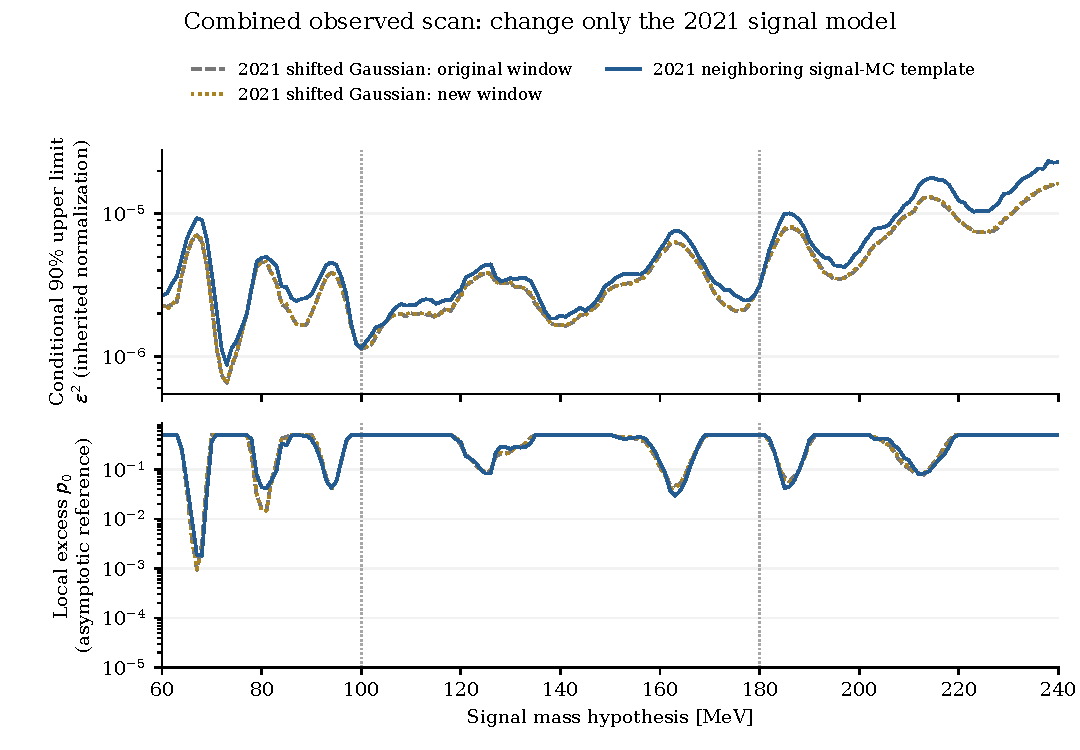
\includegraphics[width=\linewidth,height=4.65in,keepaspectratio]{../figures/v639_combined_comparison.pdf}\end{center}
{\small\textbf{Figure 1.} \textbf{How to read the figure.} All curves use the same observed campaigns and the same shared normalization. Blue changes 2021 to the neighboring MC template. Gray retains the original shifted Gaussian and its window; gold retains that Gaussian in the new MC window, separating the effect of the window from the shape change. Upper panel: 90\% bounded profile-CLs upper limits. Lower panel: local asymptotic excess p-values from the joint profile likelihood. Dotted vertical lines at 100 and 180 MeV mark the last included mass for 2015 and 2016. No uncertainty bands or global-search probabilities are shown.}\par\medskip
\begin{center}\small\begin{tabular}{lrrr}\toprule
2021 model in combination & Mass [MeV] & $Z_{
m local}$ & $p_0$\\\midrule
Gaussian, original window & 67 & 3.111 & 0.0009329\\
Gaussian, new window & 67 & 3.098 & 0.0009733\\
Neighboring signal MC & 68 & 2.910 & 0.001806\\
\bottomrule\end{tabular}\end{center}
Each table entry is that model's smallest local asymptotic p-value in the scan. The new MC-based combination peaks at 68 MeV, with $Z_{\rm local}=2.91$ and $p_0=0.00181$; the earlier shifted-Gaussian combination peaks at 67 MeV. These mass-selected minima have not been corrected for searching the mass range. A changed template can move the best mass and change both the fitted signal and its uncertainty; it need not strengthen either the observed limit or the excess.
\clearpage\section*{Appendix K. See what each campaign contributes}
\begin{center}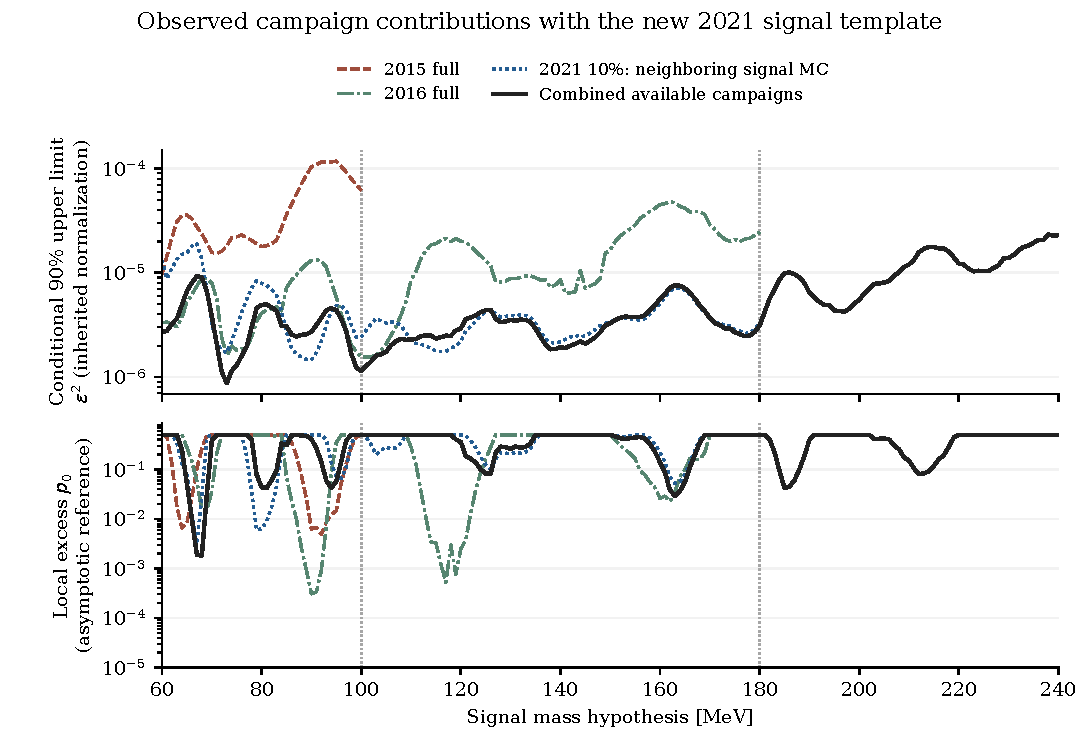
\includegraphics[width=\linewidth,height=4.65in,keepaspectratio]{../figures/v639_campaign_contributions.pdf}\end{center}
{\small\textbf{Figure 2.} \textbf{How to read the figure.} The colored curves fit each campaign separately under the same normalization convention; the black curve profiles their common signal parameter. The 2021 curve uses the neighboring MC shape. Upper panel: observed 90\% coupling-coordinate limits. Lower panel: local asymptotic excess probabilities. A campaign curve ends where its supported mass range ends. Above 180 MeV only 2021 remains, so its curve and the combined curve coincide. The dotted boundaries do not indicate candidate signal masses.}\par\medskip
\begin{center}\small\begin{tabular}{lrrr}\toprule
At 68 MeV & Signed root & $p_0$ & $\epsilon^2_{90}\ [10^{-6}]$\\\midrule
2015 full & 0.636 & 0.2624 & 23.447\\
2016 full & 2.169 & 0.01503 & 8.924\\
2021 (10\%) & 1.897 & 0.02894 & 13.424\\
Combined & 2.910 & 0.001806 & 9.046\\
\bottomrule\end{tabular}\end{center}
The signed root is positive for an excess and negative for a deficit. The upward test sets $q_0=0$ when the fitted common amplitude is negative; its conventional asymptotic reference is then $p_0=0.5$. An observed combined limit can be weaker than one campaign's limit if another campaign has an upward fluctuation. These are observed limits, not a median expected-sensitivity comparison.
\clearpage\section*{Appendix K. Validate the combined scan}

At the new combination's most significant mass, 68 MeV, generate 1,000 independent joint background-only experiments. Each campaign receives independent Poisson counts about its own archived fixed GP mean. The same complete experiment is fitted with each of the three 2021 models. GP predictions and covariance matrices are recomputed from that experiment's sidebands; the kernel parameters remain fixed.

For each method, compare the observed excess statistic $q_0=\max(r,0)^2$ with its own toy distribution. Count $k$ toys at least as extreme and report the finite-sample rank $(k+1)/1001$. The exact two-sided 95\% Clopper--Pearson interval uses denominator 1,000 and describes the underlying binomial exceedance fraction, not the add-one rank value.
\begin{center}\small\begin{tabular}{lrrl}\toprule
2021 model at 68 MeV & Count & Rank p & Exact 95\% interval\\\midrule
Neighboring signal MC & 0/1000 & 0.000999 & [0, 0.003682]\\
Gaussian, original window & 2/1000 & 0.002997 & [0.0002423, 0.007206]\\
Gaussian, new window & 0/1000 & 0.000999 & [0, 0.003682]\\
\bottomrule\end{tabular}\end{center}
No morph toy exceeds the observed statistic. This gives rank $p=1/1001$, not zero probability; the exact interval extends up to about 0.00368. The toy sample cannot determine a more precise rare-tail probability. The mass was selected using the observed scan, so this remains a fixed-mass conditional diagnostic. A global p-value would require repeating the complete mass scan in each joint toy. The earlier standalone 2021 toy calibration is not substituted for this joint check.

\textbf{Numerical validation.} The scan contains 543 new joint limit fits, 162 new individual 2015/2016 fits, and 543 inherited 2021 fits converted to the shared coordinate. All 181 original-window Gaussian joint results reproduce the earlier combined scan to numerical precision. Above 180 MeV, the new combined fits reproduce the 2021-only results. Saved replays at the strongest mass, representative masses and campaign boundaries check the joint likelihood factorization, nuisance fits and Hessian yield errors. All 3,000 selected-mass background-toy fits pass the numerical checks.

\textbf{Reproducible inputs.} The embedded \path{appendix_combined_morph/} directory contains the complete campaign spectra, frozen GP and likelihood code, v16 signal-MC inputs, scan and toy checkpoints, normalization and comparison tables, representative likelihood components, and QA. Run \path{scripts/run_combined.py} to verify or rebuild numerical results, then \path{scripts/make_figures.py} and \path{scripts/build_report.py} with \texttt{--build}. The full note preserves the preceding 52-page release separately.

\textbf{Method reference.} The fixed-mass asymptotic discovery and bounded profile-limit construction follows Cowan et al., \href{https://arxiv.org/abs/1007.1727}{arXiv:1007.1727}. The neighboring-template construction is described in Appendix J and related to Baak et al., \href{https://arxiv.org/abs/1410.7388}{arXiv:1410.7388}. These references motivate the methods; the checks above establish numerical reproducibility, not global calibration or selection-equivalence validation.

\end{document}
